\chapter{[En curso] Diseño del sistema propuesto}
\label{chapter:disenio}

\chapquote{Si tienes tanto miedo al fracaso, nunca tendrás éxito.}{Mario Andretti}

\todo[inline]{Tiene sentido llamarlo asi?}
\section{Descripción del caso de estudio} \label{section:CasoEstudio}


\section{Modelado de alto nivel}
    \subsection{Casos de uso}

\section{Diseño del sistema}

    \subsection{Arquitectura del sistema}
    \subsection{Persistencia de datos}
    \subsection{Diagramas de secuencia}
    \subsection{Interfaz de usuario}

\section{Buffer}

Tenemos las siguientes features:
\begin{enumerate}
    \item Extracción de datos de un \gls{wearable}
    \item Recopilación de histórico
    \item Seguimiento individual
    \item Seguimiento conjunto
    \item Bienvenida al usuario
\end{enumerate}

\subsection{Casos de uso}

    \subsubsection{Feature 1: Bienvenida al usuario e inicialización de la aplicación}

    \begin{table}[h]
        \centering
        \begin{tabularx}{\textwidth}{|l|l|X|}
            \hline
            01 & \multicolumn{2}{|X|}{Primer uso de la aplicación} \\
            \hline
            Evento activador & \multicolumn{2}{|X|}{El usuario abre por primera vez la aplicación} \\
            \hline
            Actor primario & \multicolumn{2}{|X|}{Usuario} \\
            \hline
            Precondición & \multicolumn{2}{|X|}{El usuario tiene instalado el \gls{framework} Salud Conectada en su dispositivo} \\
            \hline
            \multirow{10}{*}{Flujo normal} & Paso & Acción \\
            \cline{2-3} & 1 & La aplicación presenta al usuario el panel de bienvenida \\
            \cline{2-3} & 2 & El usuario finaliza u omite el panel de bienvenida \\
            \cline{2-3} & 3 & La aplicación presenta al usuario una ventana de permisos, solicitando el permiso de notificaciones y de cada tipo de dato de actividad física \\
            \cline{2-3} & 3.1 & Para cada permiso, la aplicación muestra un botón para otorgar dicho permiso y su motivación \\
            \cline{2-3} & 4 & El usuario otorga los permisos según sus preferencias \\
            \cline{2-3} & 5 & El usuario confirma su elección de permisos \\
            \cline{2-3} & 6 & La aplicación crea los canales de notificación \\
            \cline{2-3} & 7 & La aplicación planifica las tareas recurrentes \\
            \cline{2-3} & 8 & La aplicación guarda en la base de datos para cada tipo de dato de actividad física la marca de tiempo actual \\
            \hline
            Flujo alternativo & \multicolumn{2}{|X|}{Ninguno} \\
            \hline
            Postcondición & \multicolumn{2}{|X|}{El usuario es redirigido a la página principal} \\
            \hline
            Excepciones & \multicolumn{2}{|X|}{Ninguna} \\
            \hline
        \end{tabularx}
        \caption{Especificación del caso de uso 1: Primer uso de la aplicación}
        \label{tabla:casos_uso:primer_uso}
    \end{table}    
    
    \subsubsection{Feature 2: Extracción de datos de un \gls{wearable}}

    \todo[inline]{Me sale bajo un mismo caso de uso el acceso, envío y procesado de datos porque de lo contrario me quedan casos de uso sin usuario}
    \todo[inline]{No tengo claro el evento activador, si es algo que hace el usuario o viene de un actor implícito como el SO}

    \begin{table}[h]
        \centering
        \begin{tabularx}{\textwidth}{|l|l|X|}
            \hline
            02 & \multicolumn{2}{|X|}{Acceso a los datos del \gls{wearable}} \\
            \hline
            Evento activador & \multicolumn{2}{|X|}{Activación por parte de Android del procedimiento de extracción de datos} \\
            \hline
            Actor primario & \multicolumn{2}{|X|}{Usuario} \\
            \hline
            Precondición & \multicolumn{2}{|X|}{El usuario dispone de un \gls{wearable}, lo utiliza  y ha completado la fase de bienvenida} \\
            \hline
            \multirow{11}{*}{Flujo normal} & Paso & Acción \\
            \cline{2-3} & 1 & El sistema comprueba si dispone de permisos para al menos un tipo de dato \\
            \cline{2-3} & 2 & Para cada tipo de dato \\
            \cline{2-3} & 2.1 & Se comprueba el permiso de lectura \\
            \cline{2-3} & 2.2 & Si el usuario otorgó el permiso, la aplicación lee los registros del usuario de ese tipo de dato desde la última lectura registrada hasta el instante actual \\
            \cline{2-3} & 2.3 & Se procesa cada registro leído para mantener únicamente las marcas de tiempo y los datos de la propia medición \\
            \cline{2-3} & 3 & La aplicación envía al servidor la información recopilada junto al identificador de usuario \\
            \cline{2-3} & 4 & El servidor comprueba el formato de los datos enviados  \\
            \cline{2-3} & 5 & El servidor guarda en su base de datos la información recibida \\
            \cline{2-3} & 6 & El servidor envía, para cada tipo de dato, la marca de tiempo del último registro insertado en base de datos (o nulo si no se ha insertado ningún registro para ese tipo de dato) \\
            \cline{2-3} & 7 & La aplicación guarda en su base de datos las marcas de tiempo recibidas junto a su tipo de datos \\     
            \hline
            \multirow{2}{*}{Flujo alternativo} & Paso & Acción \\
            \cline{2-3} & 2.2 & Si el usuario no otorgó el permiso, se omite la lectura de ese tipo de dato \\
            \hline
            Postcondición & \multicolumn{2}{|X|}{Ninguna} \\
            \hline
            \multirow{4}{*}{Excepciones} & Paso & Acción \\
            \cline{2-3} & 1 & Si la aplicación no dispone de permiso de lectura para ningún tipo de datos, el caso de uso termina \\
            \cline{2-3} & 3 & Si no se puede enviar correctamente la información, el caso de uso termina \\
            \cline{2-3} & 4 & Si el formato de los datos enviados es inválido, el servidor envía un código de error y el caso de uso termina \\
            \hline
            \caption{Especificación del caso de uso 2: Acceso a los datos del \gls{wearable}}
            \label{tabla:casos_uso:acceso_datos}
        \end{tabularx}
    \end{table}

    \begin{table}[h]
        \centering
        \begin{tabularx}{\textwidth}{|l|l|X|}
            \hline
            03 & \multicolumn{2}{|X|}{Visualización local de los datos del \gls{wearable}} \\
            \hline
            Evento activador & \multicolumn{2}{|X|}{El usuario ha indicado visualizar sus datos del \gls{wearable}} \\
            \hline
            Actor primario & \multicolumn{2}{|X|}{Usuario} \\
            \hline
            Precondición & \multicolumn{2}{|X|}{El usuario ha completado la fase de bienvenida} \\
            \hline
            \multirow{7}{*}{Flujo normal} & Paso & Acción \\
            \cline{2-3} & 1 & La aplicación dispone al usuario un panel con cada uno de los tipos de datos disponibles \\
            \cline{2-3} & 2 & El usuario pulsa sobre el tipo de datos que quiere visualizar \\
            \cline{2-3} & 3 & La aplicación comprueba si dispone de permiso de lectura  \\
            \cline{2-3} & 4 & La aplicación lee todos los datos recopilados sobre ese tipo de datos \\
            \cline{2-3} & 5 & La aplicación procesa cada registro para dotarle de interfaz gráfica \\
            \cline{2-3} & 6 & La aplicación muestra los datos procesados \\
            \cline{2-3} & 7 & El usuario visualiza los datos hasta que bien o pulsa sobre otro tipo de dato o sale de la ventana finalizando el caso de uso \\
            \hline
            \multirow{6}{*}{Flujo alternativo} & Paso & Acción \\
            \cline{2-3} & 3 & Si la aplicación no dispone de permiso de lectura, se mostrará un botón para que el usuario pueda otorgarlo \\
            \cline{2-3} & 3.1 & Si el usuario otorga el permiso de lectura, se retoma el flujo normal en el paso 4 \\
            \cline{2-3} & 3.2 & Si el usuario no otorga el permiso de lectura, se finaliza el caso de uso \\
            \cline{2-3} & 4 & Si no hay datos recopilados, la aplicación mostrará un mensaje indicando la ausencia de datos, retomándose el flujo normal en el paso 7 \\
            \cline{2-3} & 7 & Si el usuario pulsa sobre otro tipo de dato, se retoma el flujo normal en el paso 3 \\
            \hline
            Postcondición & \multicolumn{2}{|X|}{Ninguna} \\
            \hline
            Excepciones & \multicolumn{2}{|X|}{Ninguna} \\
            \hline
            \caption{Especificación del caso de uso 3: Visualización local de los datos del \gls{wearable}}
            \label{tabla:casos_uso:visualizacion_local_wearable}
        \end{tabularx}
    \end{table}

    \begin{table}[h]
        \centering
        \begin{tabularx}{\textwidth}{|l|l|X|}
            \hline
            04 & \multicolumn{2}{|X|}{Visualización general de los datos de actividad física} \\
            \hline
            Evento activador & \multicolumn{2}{|X|}{El analista de datos ha indicado visualizar los datos generales de actividad física} \\
            \hline
            Actor primario & \multicolumn{2}{|X|}{Analista de datos} \\
            \hline
            Precondición & \multicolumn{2}{|X|}{Ninguna} \\
            \hline
            \multirow{3}{*}{Flujo normal} & Paso & Acción \\
            \cline{2-3} & 1 & El analista de datos se conecta a la base de datos del servidor \\
            \cline{2-3} & 2 & El analista de datos puede consultar para cada identificador de usuario, los datos de actividad física \\
            \hline
            Flujo alternativo & \multicolumn{2}{|X|}{Ninguno} \\
            \hline
            Postcondición & \multicolumn{2}{|X|}{Ninguna} \\
            \hline
            Excepciones & \multicolumn{2}{|X|}{Ninguna} \\
            \hline
            \caption{Especificación del caso de uso 4: Visualización general de los datos de actividad física}
            \label{tabla:casos_uso:visualizacion_general_actividad}
        \end{tabularx}
    \end{table}
    
    \subsubsection{Feature 3: Seguimiento individual}

    \begin{table}[h]
        \centering
        \begin{tabularx}{\textwidth}{|l|l|X|}
            \hline
            05 & \multicolumn{2}{|X|}{Seguimiento del estrés} \\
            \hline
            Evento activador & \multicolumn{2}{|X|}{Activación por parte de Android del procedimiento de seguimiento del estrés} \\
            \hline
            Actor primario & \multicolumn{2}{|X|}{Usuario} \\
            \hline
            Precondición & \multicolumn{2}{|X|}{El usuario ha completado la fase de bienvenida} \\
            \hline
            \multirow{13}{*}{Flujo normal} & Paso & Acción \\
            \cline{2-3} & 1 & La aplicación crea uno de los siguientes tres cuestionarios \\
            \cline{2-3} & 1.1 & Diario matutino \\
            \cline{2-3} & 1.2 & Diario vespertino \\
            \cline{2-3} & 1.3 & Puntual \\
            \cline{2-3} & 2 & La aplicación crea una notificación al usuario \\
            \cline{2-3} & 3 & El usuario pulsa en la notificación \\
            \cline{2-3} & 4 & La aplicación muestra al usuario el cuestionario \\
            \cline{2-3} & 5 & El usuario rellena el cuestionario \\
            \cline{2-3} & 6 & El usuario finaliza el cuestionario \\
            \cline{2-3} & 7 & La aplicación computa el cuestionario, obteniendo su puntuación numérica del cuestionario, el nivel categórico de estrés según el cuestionario y un consejo acorde al nivel \\
            \cline{2-3} & 8 & La aplicación muestra al usuario la puntuación numérica del cuestionario, el nivel categórico según el cuestionario y un consejo acorde al nivel \\
            \cline{2-3} & 9 & El cuestionario se guarda en base de datos \\
            \hline
            \multirow{6}{*}{Flujo alternativo} & Paso & Acción \\
            \cline{2-3} & 5 & El usuario omite la finalización del cuestionario \\
            \cline{2-3} & 5.1 & Se guarda en base de datos la información disponible del cuestionario \\
            \cline{2-3} & 5.2 & Cuando el usuario visite la página principal, se mostrará un aviso de cuestionarios incompletos para que el usuario pueda retomarlo, reanudándose el flujo normal en el paso 4 \\
            \cline{2-3} & 6 & El usuario no ha respondido a todas las preguntas \\
            \cline{2-3} & 6.1 & La aplicación muestra al usuario las preguntas restantes, reanudándose el flujo normal en el paso 5 \\
            \hline
            Postcondición & \multicolumn{2}{|X|}{La aplicación devuelve al usuario a la página principal} \\
            \hline
            \multirow{2}{*}{Excepciones}  & Paso & Acción \\
            \cline{2-3} & 2 & Si el usuario no ha indicado el permiso de notificaciones, el usuario podrá abrir el cuestionario mediante el aviso de cuestionarios incompletos de la página principal \\
            \hline
            \caption{Especificación del caso de uso 5: Seguimiento del estrés}
            \label{tabla:casos_uso:seguimiento_estres}
        \end{tabularx}
    \end{table}

    \begin{table}[h]
        \centering
        \begin{tabularx}{\textwidth}{|l|l|X|}
            \hline
            06 & \multicolumn{2}{|X|}{Seguimiento de la depresión} \\
            \hline
            Evento activador & \multicolumn{2}{|X|}{Activación por parte de Android del procedimiento de seguimiento de la depresión} \\
            \hline
            Actor primario & \multicolumn{2}{|X|}{Usuario} \\
            \hline
            Precondición & \multicolumn{2}{|X|}{El usuario ha completado la fase de bienvenida y ha permitido la monitorización de la depresión} \\
            \hline
            \multirow{13}{*}{Flujo normal} & Paso & Acción \\
            \cline{2-3} & 1 & La aplicación crea uno de los siguientes tres cuestionarios \\
            \cline{2-3} & 1.1 & Diario matutino \\
            \cline{2-3} & 1.2 & Diario vespertino \\
            \cline{2-3} & 1.3 & Puntual \\
            \cline{2-3} & 2 & La aplicación crea una notificación al usuario \\
            \cline{2-3} & 3 & El usuario pulsa en la notificación \\
            \cline{2-3} & 4 & La aplicación muestra al usuario el cuestionario \\
            \cline{2-3} & 5 & El usuario rellena el cuestionario \\
            \cline{2-3} & 6 & El usuario finaliza el cuestionario \\
            \cline{2-3} & 7 & La aplicación computa el cuestionario, obteniendo su puntuación numérica del cuestionario, el nivel categórico de estrés según el cuestionario y un consejo acorde al nivel \\
            \cline{2-3} & 8 & La aplicación muestra al usuario la puntuación numérica del cuestionario, el nivel categórico según el cuestionario y un consejo acorde al nivel \\
            \cline{2-3} & 9 & El cuestionario se guarda en base de datos \\
            \hline
            \multirow{6}{*}{Flujo alternativo} & Paso & Acción \\
            \cline{2-3} & 5 & El usuario omite la finalización del cuestionario \\
            \cline{2-3} & 5.1 & Se guarda en base de datos la información disponible del cuestionario \\
            \cline{2-3} & 5.2 & Cuando el usuario visite la página principal, se mostrará un aviso de cuestionarios incompletos para que el usuario pueda retomarlo, reanudándose el flujo normal en el paso 4 \\
            \cline{2-3} & 6 & El usuario no ha respondido a todas las preguntas \\
            \cline{2-3} & 6.1 & La aplicación muestra al usuario las preguntas restantes, reanudándose el flujo normal en el paso 5 \\
            \hline
            Postcondición & \multicolumn{2}{|X|}{La aplicación devuelve al usuario a la página principal} \\
            \hline
            \multirow{2}{*}{Excepciones}  & Paso & Acción \\
            \cline{2-3} & 2 & Si el usuario no ha indicado el permiso de notificaciones, el usuario podrá abrir el cuestionario mediante el aviso de cuestionarios incompletos de la página principal \\
            \hline
            \caption{Especificación del caso de uso 6: Seguimiento de la depresión}
            \label{tabla:casos_uso:seguimiento_depresion}
        \end{tabularx}
    \end{table}

    \begin{table}[h]
        \centering
        \begin{tabularx}{\textwidth}{|l|l|X|}
            \hline
            07 & \multicolumn{2}{|X|}{Seguimiento de la soledad} \\
            \hline
            Evento activador & \multicolumn{2}{|X|}{Activación por parte de Android del procedimiento de seguimiento de la soledad} \\
            \hline
            Actor primario & \multicolumn{2}{|X|}{Usuario} \\
            \hline
            Precondición & \multicolumn{2}{|X|}{El usuario ha completado la fase de bienvenida y ha permitido la monitorización de la soledad} \\
            \hline
            \multirow{13}{*}{Flujo normal} & Paso & Acción \\
            \cline{2-3} & 1 & La aplicación crea uno de los siguientes tres cuestionarios \\
            \cline{2-3} & 1.1 & Diario matutino \\
            \cline{2-3} & 1.2 & Diario vespertino \\
            \cline{2-3} & 1.3 & Puntual \\
            \cline{2-3} & 2 & La aplicación crea una notificación al usuario \\
            \cline{2-3} & 3 & El usuario pulsa en la notificación \\
            \cline{2-3} & 4 & La aplicación muestra al usuario el cuestionario \\
            \cline{2-3} & 5 & El usuario rellena el cuestionario \\
            \cline{2-3} & 6 & El usuario finaliza el cuestionario \\
            \cline{2-3} & 7 & La aplicación computa el cuestionario, obteniendo su puntuación numérica del cuestionario, el nivel categórico de estrés según el cuestionario y un consejo acorde al nivel \\
            \cline{2-3} & 8 & La aplicación muestra al usuario la puntuación numérica del cuestionario, el nivel categórico según el cuestionario y un consejo acorde al nivel \\
            \cline{2-3} & 9 & El cuestionario se guarda en base de datos \\
            \hline
            \multirow{6}{*}{Flujo alternativo} & Paso & Acción \\
            \cline{2-3} & 5 & El usuario omite la finalización del cuestionario \\
            \cline{2-3} & 5.1 & Se guarda en base de datos la información disponible del cuestionario \\
            \cline{2-3} & 5.2 & Cuando el usuario visite la página principal, se mostrará un aviso de cuestionarios incompletos para que el usuario pueda retomarlo, reanudándose el flujo normal en el paso 4 \\
            \cline{2-3} & 6 & El usuario no ha respondido a todas las preguntas \\
            \cline{2-3} & 6.1 & La aplicación muestra al usuario las preguntas restantes, reanudándose el flujo normal en el paso 5 \\
            \hline
            Postcondición & \multicolumn{2}{|X|}{La aplicación devuelve al usuario a la página principal} \\
            \hline
            \multirow{2}{*}{Excepciones}  & Paso & Acción \\
            \cline{2-3} & 2 & Si el usuario no ha indicado el permiso de notificaciones, el usuario podrá abrir el cuestionario mediante el aviso de cuestionarios incompletos de la página principal \\
            \hline
            \caption{Especificación del caso de uso 7: Seguimiento de la soledad}
            \label{tabla:casos_uso:seguimiento_soledad}
        \end{tabularx}
    \end{table}

    \begin{table}[h]
        \centering
        \begin{tabularx}{\textwidth}{|l|l|X|}
            \hline
            08 & \multicolumn{2}{|X|}{Realización de los cuestionarios contraste} \\
            \hline
            Evento activador & \multicolumn{2}{|X|}{Activación por parte de Android del procedimiento de cuestionarios contraste} \\
            \hline
            Actor primario & \multicolumn{2}{|X|}{Usuario} \\
            \hline
            Precondición & \multicolumn{2}{|X|}{El usuario ha completado la fase de bienvenida} \\
            \hline
            \multirow{8}{*}{Flujo normal} & Paso & Acción \\
            \cline{2-3} & 1 & La aplicación crea el cuestionario diariamente en horario vespertino \\
            \cline{2-3} & 2 & La aplicación crea una notificación al usuario \\
            \cline{2-3} & 3 & El usuario pulsa en la notificación \\
            \cline{2-3} & 4 & La aplicación muestra al usuario el cuestionario \\
            \cline{2-3} & 5 & El usuario rellena el cuestionario \\
            \cline{2-3} & 6 & El usuario finaliza el cuestionario \\
            \cline{2-3} & 7 & El cuestionario se guarda en base de datos \\
            \hline
            \multirow{6}{*}{Flujo alternativo} & Paso & Acción \\
            \cline{2-3} & 5 & El usuario omite la finalización del cuestionario \\
            \cline{2-3} & 5.1 & Se guarda en base de datos la información disponible del cuestionario \\
            \cline{2-3} & 5.2 & Cuando el usuario visite la página principal, se mostrará un aviso de cuestionarios incompletos para que el usuario pueda retomarlo, reanudándose el flujo normal en el paso 4 \\
            \cline{2-3} & 6 & El usuario no ha respondido a todas las preguntas \\
            \cline{2-3} & 6.1 & La aplicación muestra al usuario las preguntas restantes, reanudándose el flujo normal en el paso 5 \\
            \hline
            Postcondición & \multicolumn{2}{|X|}{La aplicación devuelve al usuario a la página principal} \\
            \hline
            \multirow{2}{*}{Excepciones}  & Paso & Acción \\
            \cline{2-3} & 2 & Si el usuario no ha indicado el permiso de notificaciones, el usuario podrá abrir el cuestionario mediante el aviso de cuestionarios incompletos de la página principal \\
            \hline
            \caption{Especificación del caso de uso 8: Realización de los cuestionarios contraste}
            \label{tabla:casos_uso:realizacion_contraste}
        \end{tabularx}
    \end{table}

    \begin{table}[h]
        \centering
        \begin{tabularx}{\textwidth}{|l|l|X|}
            \hline
            09 & \multicolumn{2}{|X|}{Seguimiento del riesgo de suicidio} \\
            \hline
            Evento activador & \multicolumn{2}{|X|}{Activación por parte de Android del procedimiento de seguimiento del riesgo de suicidio} \\
            \hline
            Actor primario & \multicolumn{2}{|X|}{Usuario} \\
            \hline
            Precondición & \multicolumn{2}{|X|}{El usuario ha completado la fase de bienvenida y ha permitido la monitorización de la depresión} \\
            \hline
            \multirow{11}{*}{Flujo normal} & Paso & Acción \\
            \cline{2-3} & 1 & La aplicación crea uno de los siguientes dos cuestionarios \\
            \cline{2-3} & 1.1 & Diario matutino \\
            \cline{2-3} & 2 & La aplicación crea una notificación al usuario \\
            \cline{2-3} & 3 & El usuario pulsa en la notificación \\
            \cline{2-3} & 4 & La aplicación muestra al usuario el cuestionario \\
            \cline{2-3} & 5 & El usuario rellena el cuestionario \\
            \cline{2-3} & 6 & El usuario finaliza el cuestionario \\
            \cline{2-3} & 7 & La aplicación computa el cuestionario, obteniendo el nivel de riesgo de suicidio y un consejo acorde al nivel \\
            \cline{2-3} & 8 & La aplicación muestra al usuario un consejo acorde al nivel de riesgo e suicidio \\
            \cline{2-3} & 9 & El cuestionario se guarda en base de datos \\
            \hline
            \multirow{6}{*}{Flujo alternativo} & Paso & Acción \\
            \cline{2-3} & 5 & El usuario omite la finalización del cuestionario \\
            \cline{2-3} & 5.1 & Se guarda en base de datos la información disponible del uestionario \\
            \cline{2-3} & 5.2 & Cuando el usuario visite la página principal, se mostrará un aviso e cuestionarios incompletos para que el usuario pueda retomarlo, reanudándose el flujo ormal en el paso 4 \\
            \cline{2-3} & 6 & El usuario no ha respondido a todas las preguntas \\
            \cline{2-3} & 6.1 & La aplicación muestra al usuario las preguntas restantes, eanudándose el flujo normal en el paso 5 \\
            \hline
            Postcondición & \multicolumn{2}{|X|}{La aplicación devuelve al usuario a la página rincipal} \\
            \hline
            \multirow{2}{*}{Excepciones}  & Paso & Acción \\
            \cline{2-3} & 2 & Si el usuario no ha indicado el permiso de notificaciones, el usuario podrá abrir el cuestionario mediante el aviso de cuestionarios incompletos de la página principal \\
            \hline
            \caption{Especificación del caso de uso 9: Seguimiento del riesgo de suicidio}
            \label{tabla:casos_uso:seguimiento_suicidio}
        \end{tabularx}
    \end{table}

    \begin{table}[h]
        \centering
        \begin{tabularx}{\textwidth}{|l|l|X|}
            \hline
            10 & \multicolumn{2}{|X|}{Visualización individual del estrés} \\
            \hline
            Evento activador & \multicolumn{2}{|X|}{El usuario accede a la ventana principal de la aplicación} \\
            \hline
            Actor primario & \multicolumn{2}{|X|}{Usuario} \\
            \hline
            Precondición & \multicolumn{2}{|X|}{El usuario ha completado la fase de bienvenida} \\
            \hline
            \multirow{13}{*}{Flujo normal} & Paso & Acción \\
            \cline{2-3} & 1 & La aplicación accede al último cuestionario de estrés \\
            \cline{2-3} & 2 & La aplicación muestra la puntuación de dicho cuestionario, el nivel categórico, un consejo sobre el mismo y un botón para el acceso a estadísticas más detalladas \\
            \cline{2-3} & 3 & El usuario visualiza los datos \\
            \cline{2-3} & 4 & El usuario pulsa en el botón de estadísticas más detalladas \\
            \cline{2-3} & 5.1 & La aplicación accede a los resultados de los cuestionarios de estrés del día anterior \\
            \cline{2-3} & 5.2 & La aplicación accede a los resultados de los cuestionarios de estrés de los últimos siete días \\
            \cline{2-3} & 5.3 & La aplicación accede a los resultados de los cuestionarios de estrés de la semana actual \\
            \cline{2-3} & 6.1 & La aplicación computará la media de las puntuaciones de los cuestionarios de estrés del día anterior y el nivel categórico correspondiente \\
            \cline{2-3} & 6.2 & La aplicación computará la media de las puntuaciones de los cuestionarios de estrés de los últimos siete días y el nivel categórico correspondiente \\
            \cline{2-3} & 6.3 & La aplicación computará, para cada día de la semana actual, la media de las puntuaciones de los cuestionarios de estrés \\
            \cline{2-3} & 7 & La aplicación mostrará los datos computados en el paso anterior, junto con un botón para visualizar estadísticas más detalladas \\
            \cline{2-3} & 8 & El usuario visualiza los datos hasta que sale de la ventana finalizando el caso de uso \\
            \hline
            \multirow{4}{*}{Flujo alternativo} & Paso & Acción \\
            \cline{2-3} & 2 & Si el último cuestionario de estrés no ha sido finalizado, se mostrará una puntuación y nivel nulos \\
            \cline{2-3} & 4 & El usuario finaliza la visualización de los datos saliendo de la ventana. Se termina el caso de uso \\
            \cline{2-3} & 8 & El usuario pulsa en el botón de estadísticas más detalladas, siendo redirigido a la ventana de historial \\
            \hline
            Postcondición & \multicolumn{2}{|X|}{Ninguna} \\
            \hline
            \multirow{4}{*}{Excepciones}  & Paso & Acción \\
            \cline{2-3} & 6.1 & Si no hay puntuaciones de los cuestionarios de estrés del día anterior, se asumirá media y nivel nulos \\
            \cline{2-3} & 6.2 & Si no hay puntuaciones de los cuestionarios de estrés de los últimos siete días, se asumirá media y nivel nulos \\
            \cline{2-3} & 6.3 & Si no hay puntuaciones de los cuestionarios de estrés de la semana actual, se asumirá media nula \\
            \hline
            \caption{Especificación del caso de uso 10: Visualización individual del estrés}
            \label{tabla:casos_uso:visualizacion_individual_estres}
        \end{tabularx}
    \end{table}

    \begin{table}[h]
        \centering
        \begin{tabularx}{\textwidth}{|l|l|X|}
            \hline
            11 & \multicolumn{2}{|X|}{Visualización individual de la depresión} \\
            \hline
            Evento activador & \multicolumn{2}{|X|}{El usuario accede a la ventana principal de la aplicación} \\
            \hline
            Actor primario & \multicolumn{2}{|X|}{Usuario} \\
            \hline
            Precondición & \multicolumn{2}{|X|}{El usuario ha completado la fase de bienvenida y ha permitido la monitorización de la depresión} \\
            \hline
            \multirow{13}{*}{Flujo normal} & Paso & Acción \\
            \cline{2-3} & 1 & La aplicación accede al último cuestionario de depresión \\
            \cline{2-3} & 2 & La aplicación muestra la puntuación de dicho cuestionario, el nivel categórico, un consejo sobre el mismo y un botón para el acceso a estadísticas más detalladas \\
            \cline{2-3} & 3 & El usuario visualiza los datos \\
            \cline{2-3} & 4 & El usuario pulsa en el botón de estadísticas más detalladas \\
            \cline{2-3} & 5.1 & La aplicación accede a los resultados de los cuestionarios de depresión del día anterior \\
            \cline{2-3} & 5.2 & La aplicación accede a los resultados de los cuestionarios de depresión de los últimos siete días \\
            \cline{2-3} & 5.3 & La aplicación accede a los resultados de los cuestionarios de depresión de la semana actual \\
            \cline{2-3} & 6.1 & La aplicación computará la media de las puntuaciones de los cuestionarios de depresión del día anterior y el nivel categórico correspondiente \\
            \cline{2-3} & 6.2 & La aplicación computará la media de las puntuaciones de los cuestionarios de depresión de los últimos siete días y el nivel categórico correspondiente \\
            \cline{2-3} & 6.3 & La aplicación computará, para cada día de la semana actual, la media de las puntuaciones de los cuestionarios de depresión \\
            \cline{2-3} & 7 & La aplicación mostrará los datos computados en el paso anterior, junto con un botón para visualizar estadísticas más detalladas \\
            \cline{2-3} & 8 & El usuario visualiza los datos hasta que sale de la ventana finalizando el caso de uso \\
            \hline
            \multirow{4}{*}{Flujo alternativo} & Paso & Acción \\
            \cline{2-3} & 2 & Si el último cuestionario de depresión no ha sido finalizado, se mostrará una puntuación y nivel nulos \\
            \cline{2-3} & 4 & El usuario finaliza la visualización de los datos saliendo de la ventana. Se termina el caso de uso \\
            \cline{2-3} & 8 & El usuario pulsa en el botón de estadísticas más detalladas, siendo redirigido a la ventana de historial \\
            \hline
            Postcondición & \multicolumn{2}{|X|}{Ninguna} \\
            \hline
            \multirow{4}{*}{Excepciones}  & Paso & Acción \\
            \cline{2-3} & 6.1 & Si no hay puntuaciones de los cuestionarios de depresión del día anterior, se asumirá media y nivel nulos \\
            \cline{2-3} & 6.2 & Si no hay puntuaciones de los cuestionarios de depresión de los últimos siete días, se asumirá media y nivel nulos \\
            \cline{2-3} & 6.3 & Si no hay puntuaciones de los cuestionarios de depresión de la semana actual, se asumirá media nula \\
            \hline
            \caption{Especificación del caso de uso 11: Visualización individual de la depresión}
            \label{tabla:casos_uso:visualizacion_individual_depresion}
        \end{tabularx}
    \end{table}

    \begin{table}[h]
        \centering
        \begin{tabularx}{\textwidth}{|l|l|X|}
            \hline
            12 & \multicolumn{2}{|X|}{Visualización individual de la soledad} \\
            \hline
            Evento activador & \multicolumn{2}{|X|}{El usuario accede a la ventana principal de la aplicación} \\
            \hline
            Actor primario & \multicolumn{2}{|X|}{Usuario} \\
            \hline
            Precondición & \multicolumn{2}{|X|}{El usuario ha completado la fase de bienvenida y ha permitido la monitorización de la soledad} \\
            \hline
            \multirow{13}{*}{Flujo normal} & Paso & Acción \\
            \cline{2-3} & 1 & La aplicación accede al último cuestionario de soledad \\
            \cline{2-3} & 2 & La aplicación muestra la puntuación de dicho cuestionario, el nivel categórico, un consejo sobre el mismo y un botón para el acceso a estadísticas más detalladas \\
            \cline{2-3} & 3 & El usuario visualiza los datos \\
            \cline{2-3} & 4 & El usuario pulsa en el botón de estadísticas más detalladas \\
            \cline{2-3} & 5.1 & La aplicación accede a los resultados de los cuestionarios de soledad del día anterior \\
            \cline{2-3} & 5.2 & La aplicación accede a los resultados de los cuestionarios de soledad de los últimos siete días \\
            \cline{2-3} & 5.3 & La aplicación accede a los resultados de los cuestionarios de soledad de la semana actual \\
            \cline{2-3} & 6.1 & La aplicación computará la media de las puntuaciones de los cuestionarios de soledad del día anterior y el nivel categórico correspondiente \\
            \cline{2-3} & 6.2 & La aplicación computará la media de las puntuaciones de los cuestionarios de soledad de los últimos siete días y el nivel categórico correspondiente \\
            \cline{2-3} & 6.3 & La aplicación computará, para cada día de la semana actual, la media de las puntuaciones de los cuestionarios de soledad \\
            \cline{2-3} & 7 & La aplicación mostrará los datos computados en el paso anterior, junto con un botón para visualizar estadísticas más detalladas \\
            \cline{2-3} & 8 & El usuario visualiza los datos hasta que sale de la ventana finalizando el caso de uso \\
            \hline
            \multirow{4}{*}{Flujo alternativo} & Paso & Acción \\
            \cline{2-3} & 2 & Si el último cuestionario de soledad no ha sido finalizado, se mostrará una puntuación y nivel nulos \\
            \cline{2-3} & 4 & El usuario finaliza la visualización de los datos saliendo de la ventana. Se termina el caso de uso \\
            \cline{2-3} & 8 & El usuario pulsa en el botón de estadísticas más detalladas, siendo redirigido a la ventana de historial \\
            \hline
            Postcondición & \multicolumn{2}{|X|}{Ninguna} \\
            \hline
            \multirow{4}{*}{Excepciones}  & Paso & Acción \\
            \cline{2-3} & 6.1 & Si no hay puntuaciones de los cuestionarios de soledad del día anterior, se asumirá media y nivel nulos \\
            \cline{2-3} & 6.2 & Si no hay puntuaciones de los cuestionarios de soledad de los últimos siete días, se asumirá media y nivel nulos \\
            \cline{2-3} & 6.3 & Si no hay puntuaciones de los cuestionarios de soledad de la semana actual, se asumirá media nula \\
            \hline
            \caption{Especificación del caso de uso 12: Visualización individual de la soledad}
            \label{tabla:casos_uso:visualizacion_individual_soledad}
        \end{tabularx}
    \end{table}

    
    \subsubsection{Feature 4: Seguimiento conjunto}

    \begin{table}[h]
        \centering
        \begin{tabularx}{\textwidth}{|l|l|X|}
            \hline
            13 & \multicolumn{2}{|X|}{Sincronización de datos de seguimiento} \\
            \hline
            Evento activador & \multicolumn{2}{|X|}{Activación por parte de Android del procedimiento de sincronización} \\
            \hline
            Actor primario & \multicolumn{2}{|X|}{Usuario} \\
            \hline
            Precondición & \multicolumn{2}{|X|}{El usuario ha completado la fase de bienvenida} \\
            \hline
            \multirow{8}{*}{Flujo normal} & Paso & Acción \\
            \cline{2-3} & 1 & Para cada tipo de cuestionario \\
            \cline{2-3} & 1.1 & La aplicación accede a todos los registros comprendidos entre la última sincronización registrada y el instante actual \\
            \cline{2-3} & 2 & La aplicación envía al servidor los datos recopilados junto al identificador de usuario \\
            \cline{2-3} & 3 & El servidor comprueba el formato de los datos enviados \\
            \cline{2-3} & 4 & El servidor guarda en su base de datos la información recibida \\
            \cline{2-3} & 5 & El servidor envía, para cada tipo de cuestionario, la marca de tiempo del último registro insertado en base de datos (o nulo si no se ha insertado ningún registro para ese tipo de dato) \\
            \cline{2-3} & 6 & La aplicación guarda en su base de datos las marcas de tiempo recibidas junto a su tipo de datos \\
            \hline
            Flujo alternativo & \multicolumn{2}{|X|}{Ninguno} \\
            \hline
            Postcondición & \multicolumn{2}{|X|}{Ninguna} \\
            \hline
            \multirow{3}{*}{Excepciones}  & Paso & Acción \\
            \cline{2-3} & 2 & Si no se puede enviar correctamente la información, el caso de uso termina \\
            \cline{2-3} & 3 & Si el formato de los datos enviados es inválido, el servidor envía un código de error y el caso de uso termina \\
            \hline
            \caption{Especificación del caso de uso 13: Sincronización de datos de seguimiento}
            \label{tabla:casos_uso:sincronizacion_seguimiento}
        \end{tabularx}
    \end{table}

    \begin{table}[h]
        \centering
        \begin{tabularx}{\textwidth}{|l|l|X|}
            \hline
            14 & \multicolumn{2}{|X|}{Visualización conjunta del estrés} \\
            \hline
            Evento activador & \multicolumn{2}{|X|}{El usuario accede a la ventana de visualización conjunta de estrés} \\
            \hline
            Actor primario & \multicolumn{2}{|X|}{Usuario} \\
            \hline
            Precondición & \multicolumn{2}{|X|}{El usuario ha completado la fase de bienvenida} \\
            \hline
            \multirow{6}{*}{Flujo normal} & Paso & Acción \\
            \cline{2-3} & 1 & La aplicación obtiene del servidor la media de la puntuación de los cuestionarios de estrés del día anterior, de los últimos siete días y de cada día de la semana actual \\
            \cline{2-3} & 2.1 & La aplicación muestra la media de la puntuación de los cuestionarios de estrés del día anterior y su nivel categórico \\
            \cline{2-3} & 2.2 & La aplicación muestra la media de la puntuación de los cuestionarios de estrés de los últimos siete días y su nivel categórico \\
            \cline{2-3} & 2.3 & La aplicación muestra la media de la puntuación de los cuestionarios de estrés para cada día de la semana actual \\
            \cline{2-3} & 3 & El usuario visualiza los datos hasta que sale de la ventana, finalizando el caso de uso \\
            \hline
            Flujo alternativo & \multicolumn{2}{|X|}{Ninguno} \\
            \hline
            Postcondición & \multicolumn{2}{|X|}{Ninguna} \\
            \hline
            \multirow{4}{*}{Excepciones}  & Paso & Acción \\
            \cline{2-3} & 2.1 & Si no hay puntuaciones de los cuestionarios de estrés del día anterior, se asumirá media y nivel nulos \\
            \cline{2-3} & 2.2 & Si no hay puntuaciones de los cuestionarios de estrés de los últimos siete días, se asumirá media y nivel nulos \\
            \cline{2-3} & 2.3 & Si no hay puntuaciones de los cuestionarios de estrés de la semana actual, se asumirá media nula \\
            \hline
            \caption{Especificación del caso de uso 14: Visualización conjunta del estrés}
            \label{tabla:casos_uso:visualizacion_conjunta_estres}
        \end{tabularx}
    \end{table}

    \begin{table}[h]
        \centering
        \begin{tabularx}{\textwidth}{|l|l|X|}
            \hline
            15 & \multicolumn{2}{|X|}{Visualización conjunta de la depresión} \\
            \hline
            Evento activador & \multicolumn{2}{|X|}{El usuario accede a la ventana de visualización conjunta de depresión} \\
            \hline
            Actor primario & \multicolumn{2}{|X|}{Usuario} \\
            \hline
            Precondición & \multicolumn{2}{|X|}{El usuario ha completado la fase de bienvenida y ha permitido la monitorización de la depresión} \\
            \hline
            \multirow{6}{*}{Flujo normal} & Paso & Acción \\
            \cline{2-3} & 1 & La aplicación obtiene del servidor la media de la puntuación de los cuestionarios de depresión del día anterior, de los últimos siete días y de cada día de la semana actual \\
            \cline{2-3} & 2.1 & La aplicación muestra la media de la puntuación de los cuestionarios de depresión del día anterior y su nivel categórico \\
            \cline{2-3} & 2.2 & La aplicación muestra la media de la puntuación de los cuestionarios de depresión de los últimos siete días y su nivel categórico \\
            \cline{2-3} & 2.3 & La aplicación muestra la media de la puntuación de los cuestionarios de depresión para cada día de la semana actual \\
            \cline{2-3} & 3 & El usuario visualiza los datos hasta que sale de la ventana, finalizando el caso de uso \\
            \hline
            Flujo alternativo & \multicolumn{2}{|X|}{Ninguno} \\
            \hline
            Postcondición & \multicolumn{2}{|X|}{Ninguna} \\
            \hline
            \multirow{4}{*}{Excepciones}  & Paso & Acción \\
            \cline{2-3} & 2.1 & Si no hay puntuaciones de los cuestionarios de depresión del día anterior, se asumirá media y nivel nulos \\
            \cline{2-3} & 2.2 & Si no hay puntuaciones de los cuestionarios de depresión de los últimos siete días, se asumirá media y nivel nulos \\
            \cline{2-3} & 2.3 & Si no hay puntuaciones de los cuestionarios de depresión de la semana actual, se asumirá media nula \\
            \hline
            \caption{Especificación del caso de uso 15: Visualización conjunta de la depresión}
            \label{tabla:casos_uso:visualizacion_conjunta_depresion}
        \end{tabularx}
    \end{table}

    \begin{table}[h]
        \centering
        \begin{tabularx}{\textwidth}{|l|l|X|}
            \hline
            16 & \multicolumn{2}{|X|}{Visualización conjunta de la soledad} \\
            \hline
            Evento activador & \multicolumn{2}{|X|}{El usuario accede a la ventana de visualización conjunta de soledad} \\
            \hline
            Actor primario & \multicolumn{2}{|X|}{Usuario} \\
            \hline
            Precondición & \multicolumn{2}{|X|}{El usuario ha completado la fase de bienvenida y ha permitido la monitorización de la soledad} \\
            \hline
            \multirow{6}{*}{Flujo normal} & Paso & Acción \\
            \cline{2-3} & 1 & La aplicación obtiene del servidor la media de la puntuación de los cuestionarios de soledad del día anterior, de los últimos siete días y de cada día de la semana actual \\
            \cline{2-3} & 2.1 & La aplicación muestra la media de la puntuación de los cuestionarios de soledad del día anterior y su nivel categórico \\
            \cline{2-3} & 2.2 & La aplicación muestra la media de la puntuación de los cuestionarios de soledad de los últimos siete días y su nivel categórico \\
            \cline{2-3} & 2.3 & La aplicación muestra la media de la puntuación de los cuestionarios de soledad para cada día de la semana actual \\
            \cline{2-3} & 3 & El usuario visualiza los datos hasta que sale de la ventana, finalizando el caso de uso \\
            \hline
            Flujo alternativo & \multicolumn{2}{|X|}{Ninguno} \\
            \hline
            Postcondición & \multicolumn{2}{|X|}{Ninguna} \\
            \hline
            \multirow{4}{*}{Excepciones}  & Paso & Acción \\
            \cline{2-3} & 2.1 & Si no hay puntuaciones de los cuestionarios de soledad del día anterior, se asumirá media y nivel nulos \\
            \cline{2-3} & 2.2 & Si no hay puntuaciones de los cuestionarios de soledad de los últimos siete días, se asumirá media y nivel nulos \\
            \cline{2-3} & 2.3 & Si no hay puntuaciones de los cuestionarios de soledad de la semana actual, se asumirá media nula \\
            \hline
            \caption{Especificación del caso de uso 16: Visualización conjunta de la soledad}
            \label{tabla:casos_uso:visualizacion_conjunta_soledad}
        \end{tabularx}
    \end{table}

    \begin{table}[h]
        \centering
        \begin{tabularx}{\textwidth}{|l|l|X|}
            \hline
            17 & \multicolumn{2}{|X|}{Visualización general de los datos de seguimiento} \\
            \hline
            Evento activador & \multicolumn{2}{|X|}{El analista de datos ha indicado visualizar los datos generales de seguimiento} \\
            \hline
            Actor primario & \multicolumn{2}{|X|}{Analista de datos} \\
            \hline
            Precondición & \multicolumn{2}{|X|}{Ninguna} \\
            \hline
            \multirow{3}{*}{Flujo normal} & Paso & Acción \\
            \cline{2-3} & 1 & El analista de datos se conecta a la base de datos del servidor \\
            \cline{2-3} & 2 & El analista de datos puede consultar para cada identificador de usuario, los datos de los cuestionarios realizados \\
            \hline
            Flujo alternativo & \multicolumn{2}{|X|}{Ninguno} \\
            \hline
            Postcondición & \multicolumn{2}{|X|}{Ninguna} \\
            \hline
            Exepciones & \multicolumn{2}{|X|}{Ninguna} \\
            \hline
            \caption{Especificación del caso de uso 17: Visualización general de los datos de seguimiento}
            \label{tabla:casos_uso:visualizacion_general_seguimiento}
        \end{tabularx}
    \end{table}

    \subsubsection{Feature 5: Recopilación del histórico}

    \begin{table}[h]
        \centering
        \begin{tabularx}{\textwidth}{|l|l|X|}
            \hline
            18 & \multicolumn{2}{|X|}{Visualización estadística de los datos de estrés} \\
            \hline
            Evento activador & \multicolumn{2}{|X|}{El usuario accede a la ventana de histórico de la aplicación} \\
            \hline
            Actor primario & \multicolumn{2}{|X|}{Usuario} \\
            \hline
            Precondición & \multicolumn{2}{|X|}{El usuario ha completado la fase de bienvenida} \\
            \hline
            \multirow{7}{*}{Flujo normal} & Paso & Acción \\
            \cline{2-3} & 1 & La aplicación asume por defecto que los datos se agruparán por día y el intervalo de fechas son los últimos siete días \\
            \cline{2-3} & 2 & La aplicación acede a los datos de los cuestionarios de estrés del intervalo de fechas \\
            \cline{2-3} & 3 & La aplicación procesa los datos leídos, agrupando los datos según la granularidad y realizando la media \\
            \cline{2-3} & 4 & La aplicación presenta los datos procesados \\
            \cline{2-3} & 5 & El usuario visualiza los datos \\
            \cline{2-3} & 6 & El usuario finaliza la visualización de los datos \\
            \hline
            \multirow{5}{*}{Flujo alternativo} & Paso & Acción \\
            \cline{2-3} & 3 & Si en alguna de las agrupaciones no hay datos con lo que realizar la media, se realiza la siguiente imputación \\
            \cline{2-3} & 3.1 & Si hay datos en las tres agrupaciones previas, se realiza la media de la puntuación de estas \\
            \cline{2-3} & 3.2 & Si no hay datos en las tres agrupaciones previas, se realiza la media de la puntuación de todas las agrupaciones que tengan datos \\
            \cline{2-3} & 6 & El usuario puede cambiar la granularidad de los datos, volviendo al paso 3 del flujo normal; o el intervalo de fechas, volviendo al paso 2 del flujo normal \\
            \hline
            Postcondición & \multicolumn{2}{|X|}{Ninguna} \\
            \hline
            Exepciones & \multicolumn{2}{|X|}{Ninguna} \\
            \hline
            \caption{Especificación del caso de uso 18: Visualización estadística de los datos de estrés}
            \label{tabla:casos_uso:visualizacion_estadistica_estres}
        \end{tabularx}
    \end{table}

    \begin{table}[h]
        \centering
        \begin{tabularx}{\textwidth}{|l|l|X|}
            \hline
            19 & \multicolumn{2}{|X|}{Visualización estadística de los datos de depresión} \\
            \hline
            Evento activador & \multicolumn{2}{|X|}{El usuario accede a la ventana de histórico de la aplicación} \\
            \hline
            Actor primario & \multicolumn{2}{|X|}{Usuario} \\
            \hline
            Precondición & \multicolumn{2}{|X|}{El usuario ha completado la fase de bienvenida y ha permitido la monitorización de la depresión} \\
            \hline
            \multirow{7}{*}{Flujo normal} & Paso & Acción \\
            \cline{2-3} & 1 & La aplicación asume por defecto que los datos se agruparán por día y el intervalo de fechas son los últimos siete días \\
            \cline{2-3} & 2 & La aplicación acede a los datos de los cuestionarios de depresión del intervalo de fechas \\
            \cline{2-3} & 3 & La aplicación procesa los datos leídos, agrupando los datos según la granularidad y realizando la media \\
            \cline{2-3} & 4 & La aplicación presenta los datos procesados \\
            \cline{2-3} & 5 & El usuario visualiza los datos \\
            \cline{2-3} & 6 & El usuario finaliza la visualización de los datos \\
            \hline
            \multirow{5}{*}{Flujo alternativo} & Paso & Acción \\
            \cline{2-3} & 3 & Si en alguna de las agrupaciones no hay datos con lo que realizar la media, se realiza la siguiente imputación \\
            \cline{2-3} & 3.1 & Si hay datos en las tres agrupaciones previas, se realiza la media de la puntuación de estas \\
            \cline{2-3} & 3.2 & Si no hay datos en las tres agrupaciones previas, se realiza la media de la puntuación de todas las agrupaciones que tengan datos \\
            \cline{2-3} & 6 & El usuario puede cambiar la granularidad de los datos, volviendo al paso 3 del flujo normal; o el intervalo de fechas, volviendo al paso 2 del flujo normal \\
            \hline
            Postcondición & \multicolumn{2}{|X|}{Ninguna} \\
            \hline
            Exepciones & \multicolumn{2}{|X|}{Ninguna} \\
            \hline
            \caption{Especificación del caso de uso 19: Visualización estadística de los datos de depresión}
            \label{tabla:casos_uso:visualizacion_estadistica_depresion}
        \end{tabularx}
    \end{table}

    \begin{table}[h]
        \centering
        \begin{tabularx}{\textwidth}{|l|l|X|}
            \hline
            20 & \multicolumn{2}{|X|}{Visualización estadística de los datos de soledad} \\
            \hline
            Evento activador & \multicolumn{2}{|X|}{El usuario accede a la ventana de histórico de la aplicación} \\
            \hline
            Actor primario & \multicolumn{2}{|X|}{Usuario} \\
            \hline
            Precondición & \multicolumn{2}{|X|}{El usuario ha completado la fase de bienvenida y ha permitido la monitorización de la soledad} \\
            \hline
            \multirow{7}{*}{Flujo normal} & Paso & Acción \\
            \cline{2-3} & 1 & La aplicación asume por defecto que los datos se agruparán por día y el intervalo de fechas son los últimos siete días \\
            \cline{2-3} & 2 & La aplicación acede a los datos de los cuestionarios de soledad del intervalo de fechas \\
            \cline{2-3} & 3 & La aplicación procesa los datos leídos, agrupando los datos según la granularidad y realizando la media \\
            \cline{2-3} & 4 & La aplicación presenta los datos procesados \\
            \cline{2-3} & 5 & El usuario visualiza los datos \\
            \cline{2-3} & 6 & El usuario finaliza la visualización de los datos \\
            \hline
            \multirow{5}{*}{Flujo alternativo} & Paso & Acción \\
            \cline{2-3} & 3 & Si en alguna de las agrupaciones no hay datos con lo que realizar la media, se realiza la siguiente imputación \\
            \cline{2-3} & 3.1 & Si hay datos en las tres agrupaciones previas, se realiza la media de la puntuación de estas \\
            \cline{2-3} & 3.2 & Si no hay datos en las tres agrupaciones previas, se realiza la media de la puntuación de todas las agrupaciones que tengan datos \\
            \cline{2-3} & 6 & El usuario puede cambiar la granularidad de los datos, volviendo al paso 3 del flujo normal; o el intervalo de fechas, volviendo al paso 2 del flujo normal \\
            \hline
            Postcondición & \multicolumn{2}{|X|}{Ninguna} \\
            \hline
            Exepciones & \multicolumn{2}{|X|}{Ninguna} \\
            \hline
            \caption{Especificación del caso de uso 20: Visualización estadística de los datos de soledad}
            \label{tabla:casos_uso:visualizacion_estadistica_soledad}
        \end{tabularx}
    \end{table}

\subsection{Diagramas de secuencia}

    \subsubsection{Diagramas de secuencia 1: Extracción de datos de un \gls{wearable}}
        La secuencia lógica de la extracción de datos de un \gls{wearable} es la siguiente (Figura X):

        \begin{enumerate}
            \item Hola
            \item Mundo
            \item Bifurcación
            \begin{enumerate}
                \item Primario
                \item Alternativo
            \end{enumerate}
        \end{enumerate}
    
    \subsubsection{Diagramas de secuencia 2: Seguimiento individual}
        La secuencia lógica del seguimiento individual es la siguiente (Figura X):

        \begin{enumerate}
            \item Hola
            \item Mundo
            \item Bifurcación
            \begin{enumerate}
                \item Primario
                \item Alternativo
            \end{enumerate}
        \end{enumerate}
    
    \subsubsection{Diagramas de secuencia 3: Seguimiento conjunto}
        La secuencia lógica del seguimiento conjunto es la siguiente (Figura X):

        \begin{enumerate}
            \item Hola
            \item Mundo
            \item Bifurcación
            \begin{enumerate}
                \item Primario
                \item Alternativo
            \end{enumerate}
        \end{enumerate}
        
    \subsubsection{Diagramas de secuencia 4: Recopilación del histórico?}
        La secuencia lógica de la recopilación del histórico es la siguiente (Figura X):

        \begin{enumerate}
            \item Hola
            \item Mundo
            \item Bifurcación
            \begin{enumerate}
                \item Primario
                \item Alternativo
            \end{enumerate}
        \end{enumerate}

    \subsubsection{[WIP] Diagramas de secuencia 5: Post cuestionario}
        La secuencia lógica de la recopilación del histórico es la siguiente (Figura X):

        \begin{enumerate}
            \item Android invoca a la tarea \textit{Upload}
            \item Se comprobará si hay datos de estrés pendientes de enviar.
            \item Si hay datos pendientes de est
            \item Bifurcación
            \begin{enumerate}
                \item Primario
                \item Alternativo
            \end{enumerate}
        \end{enumerate}

Diagrama ER

\begin{sidewaysfigure}[h]
    \centering
    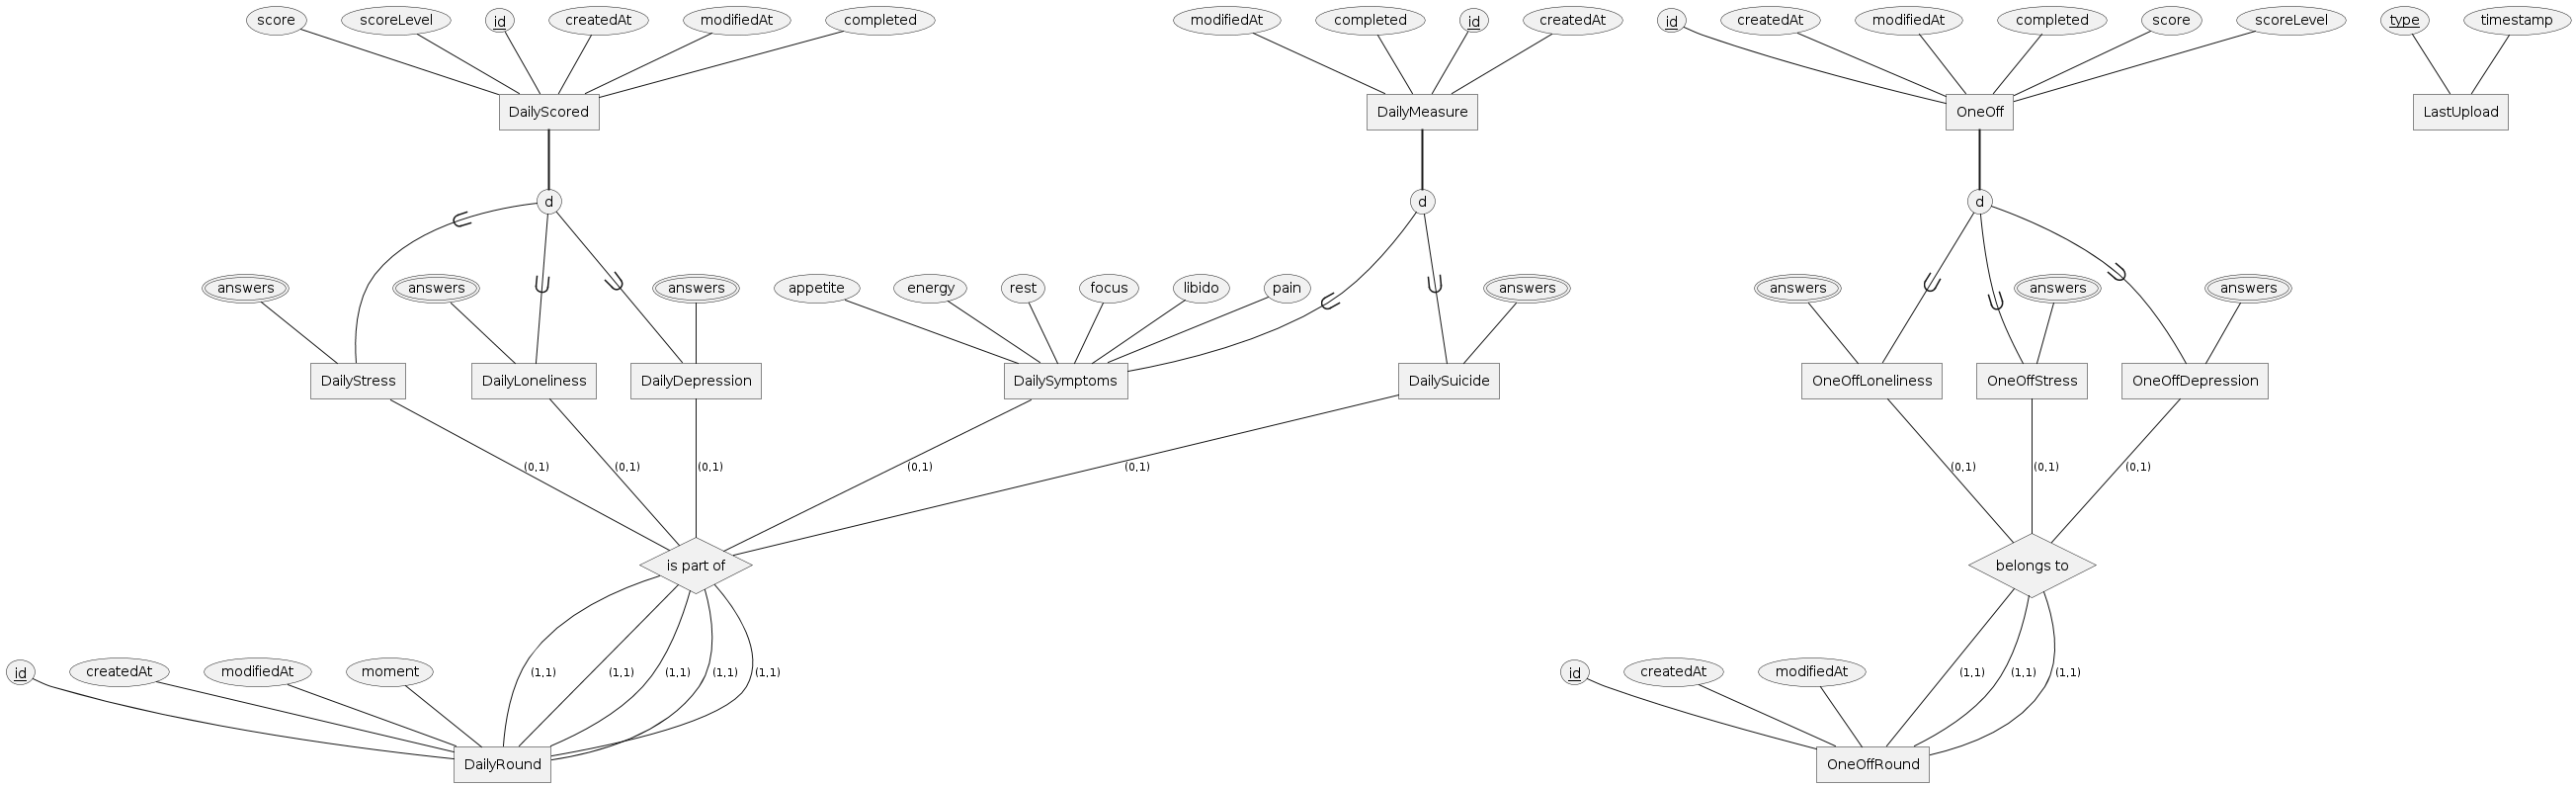
\includegraphics[width=1\textwidth]{figures/bd/ER simple.png}
    \caption[Diagrama ER]{Diagrama ER. Elaboración propia}
    \label{figure:disenio:diagrama_er}
\end{sidewaysfigure}

Diagrama colección datos usuario (\textit{user data})

\begin{figure}[h]
    \centering
    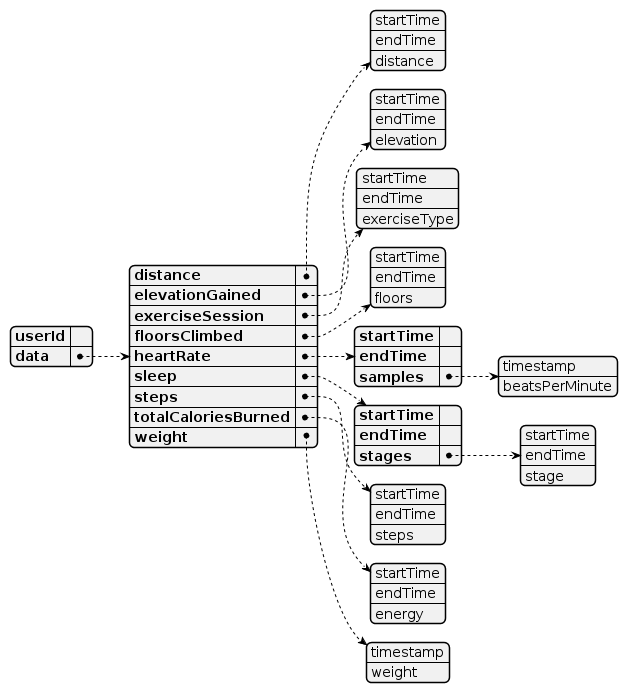
\includegraphics[width=0.75\textwidth]{figures/bd/Servidor user data.png}
    \caption[Diagrama colección datos usuario]{Diagrama colección datos usuario. Elaboración propia}
    \label{figure:disenio:diagrama_user_data}
\end{figure}

Diagrama colección cuestionarios diarios (\textit{daily questionnaires})

\begin{figure}[h]
    \centering
    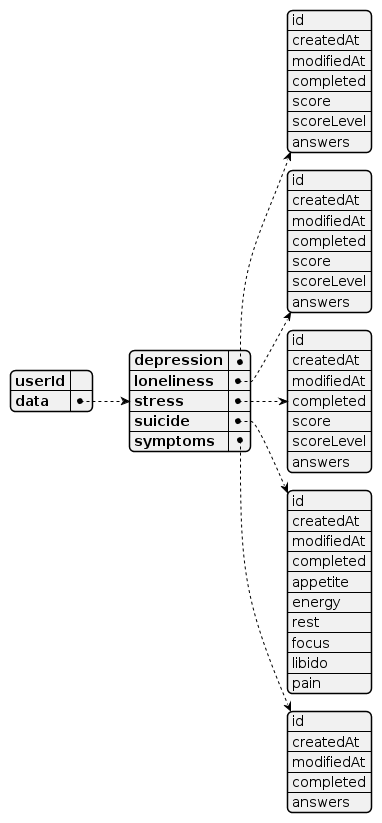
\includegraphics[width=0.33\textwidth]{figures/bd/Servidor daily questionnaires.png}
    \caption[Diagrama colección cuestionarios diarios]{Diagrama colección cuestionarios diarios. Elaboración propia}
    \label{figure:disenio:diagrama_daily}
\end{figure}

Diagrama colección cuestionarios puntuales(\textit{one off questionnaires})

\begin{figure}[h]
    \centering
    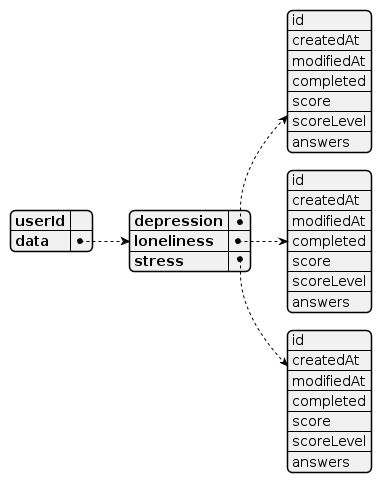
\includegraphics[width=0.33\textwidth]{figures/bd/Servidor one off questionnaires.png}
    \caption[Diagrama colección cuestionarios puntuales]{Diagrama colección cuestionarios puntuales. Elaboración propia}
    \label{figure:disenio:diagrama_one_off}
\end{figure}

\subsection{Grafos de navegación}
    \begin{figure}[h]
        \centering
        \begin{tikzpicture}[
                > = stealth, % estilo de la cabeza de la flecha
                shorten > = 1pt, % para que la flecha no toque el nodo
                node distance = 3cm, % distancia entre nodos
            ]
    
            \tikzstyle{every state}=[
                draw = black,
                thick,
                fill = white,
            ]

            \node[rectangle,draw] (click) {\textit{El usuario entra en la app}};
            \node[state] [below of=click] (splash) {Splash};
            \node[state] [below of=splash] (bienvenida) {Bienvenida};
            \node[state] [below of=bienvenida] (permisos) {Permisos};
            \node[state] [below of=permisos] (inicio) {\textit{Inicio}};
            
            \path[->] (click) edge node {} (splash);
            \path[->] (splash) edge node {} (bienvenida);
            \path[->] (bienvenida) edge node {} (permisos);
            \path[->] (permisos) edge node {} (inicio);
    
        \end{tikzpicture}
        \caption{Grafo de navegación en el primer uso de la app}
        \label{figure:disenio:grafo_primer_uso}
    \end{figure}
    
    \begin{figure}[h]
        \centering
        \begin{tikzpicture}[
                font=\small, % fuente de letra pequeña
                > = stealth, % estilo de la cabeza de la flecha
                shorten > = 1pt, % para que la flecha no toque el nodo
                node distance = 3.3cm, % distancia entre nodos
            ]
    
            \tikzstyle{every state}=[
                draw = black,
                thick,
                fill = white,
            ]

            \node[rectangle,draw] (click) {E\textit{l usuario entra en la app}};
            \node[state] [below of=click] (splash) {Splash};
            \node[state] [below of=splash] (inicio) {Inicio};
    
            \node[state] [below left of=inicio] (historial) {Historial};
            \node[state] [below right of=inicio] (comunidad) {Comunidad};
            \node[state, align=center] [right of=inicio] (incompletos) {Cuestionarios\\incompletos};
            \node[state] [below right of=historial] (ajustes) {Ajustes};
            \node[state] [left of=inicio] (consejo) {Consejo};
            \node[state] [left of=historial] (medida) {Medida};
        
            \node[state, align=center] [above right of=incompletos] (diaria) {\textit{Ronda}\\\textit{diaria}};
            \node[state, align=center] [below right of=incompletos] (puntual) {\textit{Ronda}\\\textit{puntual}};
            
            \node[state] [below of=ajustes] (bienvenida) {Bienvenida};
            \node[state] [left of=bienvenida] (mis_datos) {Mis datos};
            \node[state] [left of=mis_datos] (privacidad) {Privacidad};
            \node[state] [right of=bienvenida] (acerca) {Acerca de};
            \node[state] [right of=acerca] (créditos) {Créditos};

            \path[->] (click) edge node {} (splash);
            \path[->] (splash) edge node {} (inicio);
            
            \path[<->] (inicio) edge node {} (historial);
            \path[<->] (inicio) edge node {} (comunidad);
            \path[<->] (inicio) edge node {} (ajustes);
            \path[<->] (inicio) edge node {} (medida);
            \path[<->] (inicio) edge node {} (consejo);
            \path[<->, dashed] (inicio) edge node {} (incompletos);
    
            \path[<->] (historial) edge node {} (medida);
            \path[<->] (historial) edge node {} (comunidad);
            \path[<->] (historial) edge node {} (ajustes);
            
            \path[<->] (ajustes) edge node {} (comunidad);
            \path[<->] (ajustes) edge node {} (bienvenida);
            \path[<->] (ajustes) edge node {} (mis_datos);
            \path[<->] (ajustes) edge node {} (privacidad);
            \path[<->] (ajustes) edge node {} (acerca);
            \path[<->] (ajustes) edge node {} (créditos);
            
            \path[->] (incompletos) edge node {} (diaria);
            \path[->] (incompletos) edge node {} (puntual);
    
        \end{tikzpicture}
        \caption{Grafo de navegación principal de la app}
        \label{figure:disenio:grafo_principal}
    \end{figure}

    \begin{figure}[h]
        \centering
        \begin{tikzpicture}[
                font=\small, % fuente de letra pequeña
                > = stealth, % estilo de la cabeza de la flecha
                shorten > = 1pt, % para que la flecha no toque el nodo
                node distance = 3cm, % distancia entre nodos
            ]

            \tikzstyle{every state}=[
                draw = black,
                thick,
                fill = white,
            ]

            \node[state, align=center] (diaria) {Ronda\\diaria}; 

            \node[rectangle,draw, align=center] [above left of=diaria] (notificacion) {\textit{El usuario pulsa}\\\textit{en la notificación}};
            \node[rectangle,draw, align=center] [above right of=diaria] (incompletos) {\textit{El usuario pulsa en un} \\ \textit{cuestionario incompleto}};
            
            \node[state] [right of=diaria] (inicio) {\textit{Inicio}}; 
            
            \node[state, align=center] [below of=diaria] (suicidio_diario) {Suicidio\\diario};
            \node[state, align=center] [left of=suicidio_diario] (depresion_diario) {Depresión\\diario};
            \node[state, align=center] [left of=depresion_diario] (estres_diario) {Estrés\\diario};
            \node[state, align=center] [right of=suicidio_diario] (soledad_diario) {Soledad\\diario};
            \node[state, align=center] [right of=soledad_diario] (contraste_diario) {Contraste\\ diario};
    
            \node[state] [below of=suicidio_diario] (consejo) {Consejo};

            \path[->] (notificacion) edge node {} (diaria);
            \path[->] (incompletos) edge node {} (diaria);
            \path[->] (diaria) edge node {} (inicio);
            \path[<->,dashed] (diaria) edge node {} (estres_diario);
            \path[<->,dashed] (diaria) edge node {} (depresion_diario);
            \path[<->,dashed] (diaria) edge node {} (soledad_diario);
            \path[<->,dashed] (diaria) edge node {} (suicidio_diario);
            \path[<->,dashed] (diaria) edge node {} (contraste_diario);
    
            
            \path[<->] (consejo) edge node {} (estres_diario);
            \path[<->] (consejo) edge node {} (depresion_diario);
            \path[<->] (consejo) edge node {} (soledad_diario);
            \path[<->] (consejo) edge node {} (suicidio_diario);

        \end{tikzpicture}
        \caption{Grafo de navegación en los cuestionarios diarios de la app}
        \label{figure:disenio:grafo_diario}
    \end{figure}

    \begin{figure}[h]
        \centering
        \begin{tikzpicture}[
                font=\small, % fuente de letra pequeña
                > = stealth, % estilo de la cabeza de la flecha
                shorten > = 1pt, % para que la flecha no toque el nodo
                node distance = 3.5cm, % distancia entre nodos
            ]

            \tikzstyle{every state}=[
                draw = black,
                thick,
                fill = white,
            ]
            
            \node[state, align=center] (puntual) {Ronda\\puntual}; 
            
            \node[rectangle,draw, align=center] [above left of=diaria] (notificacion) {\textit{El usuario pulsa}\\\textit{en la notificación}};
            \node[rectangle,draw, align=center] [above right of=diaria] (incompletos) {\textit{El usuario pulsa en un} \\ \textit{cuestionario incompleto}};
            
            \node[state] [right of=diaria] (inicio) {\textit{Inicio}}; 
            
            \node[state, align=center] [below of=puntual] (depresion_puntual) {Depresión\\puntual};
            \node[state, align=center] [left of=depresion_puntual] (estres_puntual) {Estrés\\puntual};
            \node[state, align=center] [right of=depresion_puntual] (soledad_puntual) {Soledad\\puntual};
    
            \node[state] [below of=depresion_puntual] (consejo) {Consejo};
    
            \path[->] (puntual) edge node {} (inicio);
            \path[->] (notificacion) edge node {} (puntual);
            \path[->] (incompletos) edge node {} (puntual);
            
            \path[<->,dashed] (puntual) edge node {} (estres_puntual);
            \path[<->,dashed] (puntual) edge node {} (depresion_puntual);
            \path[<->,dashed] (puntual) edge node {} (soledad_puntual);
    
            \path[<->] (consejo) edge node {} (estres_puntual);
            \path[<->] (consejo) edge node {} (depresion_puntual);
            \path[<->] (consejo) edge node {} (soledad_puntual);

        \end{tikzpicture}
        \caption{Grafo de navegación en los cuestionarios puntuales de la app}
        \label{figure:disenio:grafo_puntuales}
    \end{figure}